\chapter{Funktionsuntersuchung}

Die \textbf{Analysis} (griechisch  análysis, deutsch "`Aufl"osung"') ist ein Teilgebiet der Mathematik.  Die Untersuchung von reellen und komplexen Funktionen hinsichtlich Stetigkeit, Differenzierbarkeit und Integrierbarkeit z"ahlt zu den Hauptgegenst"anden der Analysis. Die hierzu entwickelten Methoden sind in allen Natur- und Ingenieurwissenschaften von großer Bedeutung.\\

\section{Stetigkeit}

Eine Funktion ist stetig an der Stelle $x_{0}$, wenn:
\begin{enumerate}
\item $x_{0}\in D$
\item $\lim\limits_{x \rightarrow x_{0}} {f(x)}$ existiert 
\item $\lim\limits_{x \rightarrow x_{0}^{\pm}} {f(x)}=f(x_{0})$\\
\end{enumerate}
Stetigkeit ist eine lokale Eigenschaft. Die Funktion $f$ hei�t dann stetig, wenn sie an jeder Stelle ihrer Definitionsmenge stetig ist.

\begin{Bemerkung}
Ist $f$ stetig und $I\subset \R$ ein reelles Intevall, dann ist $f(I)$ ebenfalls ein Intervall. Ist $f$ zudem streng monoton, so ist die Umkehrfunktion $f^{-1}$ ebenfalls stetig.
\end{Bemerkung}

\subsubsection{Stetige Fortsetzungen}

beim Vereinfachen von gebrochenrationalen Funktionen ist Vorsicht geboten, denn eine hebbare Definitionsl�cke ''aufzuheben" ver"andert den Definitionsbereich der Funktion. Die daraus resultierende Funktion wird \textbf{stetige Fortsetzung} genannt.

\section{Differenzierbarkeit}

Eine Funktion ist differenzierbar an der Stelle $x_{0} \in D$, wenn der beitseitige Grenzwert des Differenzenquotienten f"ur $h\rightarrow 0$ existiert. Anschaulich soll Die Funktion links und rechts des $x_{0}$ die selbe Ableitung haben. \\ 
\\
$\lim\limits_{h \rightarrow 0^{+}} {\dfrac{f(x_{0}+h)-f(x_{0})}{h}} = \lim\limits_{h \rightarrow 0^{-}} {\dfrac{f(x_{0}+h)-f(x_{0})}{h}} =f'(x_{0})$\\
\\
Dieser Grenzwert ist die \textbf{Ableitung} von $f$ an der Stelle $x_{0}$.\\
Die Funktion hei�t differenzierbar, wenn sie $\forall x \in D$ differenzierbar ist.\\
\\
Die Funktion $f(x)=|x|$ ist nicht differenzierbar, da bei der Stelle $x_{0}=0$ der linksseitige Grenzwert des differenzenquotienten ($\lim\limits_{h \rightarrow 0^{-}}{f'(x_{0})=-1$}) nicht mit dem rechtsseitigen Grenzwert (1) �bereinstimmt.\\

\subsection{Zusammenhang zwischen Stetigkeit und Differenzierbarkeit}

Ist eine Funktion $f$ an der Stelle $x_{0}$ differenzierbar, so ist sie an dieser Stelle auch stetig.
Die Umkehrung gilt erst einmal nicht, aber es gibt eine verneinende Aussage: Ist $f$ an der Stelle $x_{0}$ nicht stetig, so ist sie hier auch nicht differenzierbar.\\

\section{Ableitungsregeln}


Ein Ableitungswert gibt die Steigung an einem bestimmten Punkt an. Im Allgemeinen und zum Beweisen wird der Differentenquotient ben"otigt, um eine Ableitungsfunktion zu definieren, es geht aber in vielen F"allen schneller.

\subsection{Produktregel}

Sind die Funktionen $u$ und $v$ an der Stelle $x_{0}$ $\in$ $D$ differenzierbar, dann ist die Funktion $f(x)=u(x)\cdot v(x)$ bei $x_{0}$ auch differenzierbar und es gilt: \\
\\
$f'(x0) = u'(x_{0})v(x_{0})+u(x_{0})v'(x_{0})$\\

\begin{Beweis}
$
\begin{array}{rcl}
\lim\limits_{h \rightarrow 0} {\dfrac{f(x_{0}+h)-f(x_{0})}{h}} & = & \lim\limits_{h \rightarrow 0} {\dfrac{u(x_{0})v({x_{0}+h)-u(x_{0})v(x_{0})}}{h}}\\
&=&\lim\limits_{h \rightarrow 0} {\dfrac{u(x_{0}+h)v(x_{0}+h)\textcolor{red}{-u(x_{0})v(x_{0}+h)+u(x_{0})v(x_{0}+h)}-u(x_{0})v(x_{0}) }{h}}\\
&=&\lim\limits_{h \rightarrow 0} {\dfrac{u(x_{0}+h)v(x_{0}+h)-u(x_{0})v(x_{0}+h)}{h}} + \lim\limits_{h \rightarrow 0} {\dfrac{u(x_{0})v(x_{0}+h)-u(x_{0})v(x_{0})}{h}}\\
&=&\lim\limits_{h \rightarrow 0} {v(x_{0}+h)\dfrac{u(x_{0}+h)-u(x_{0})}{h}} \lim\limits_{h \rightarrow 0} {u(x_{0})\dfrac{v(x_{0}+h)-v(x_{0})}{h}}\\
&=& v(x_{0})\lim\limits_{h \rightarrow 0}{\dfrac{u(x_{0}+h)-u(x_{0})}{h}} +u(x_{0}) \lim\limits_{h \rightarrow 0} {\dfrac{v(x_{0}+h)-v(x_{0})}{h}}\\
&=& u'(x_{0})v(x_{0}) - u(x_{0})v'(x_{0}) 
\end{array}
$
\end{Beweis}

\subsection{Quotientenregel}

Sind die Funktionen $u$ und $v$ an der Stelle $x_{0}$ $\in$ $D$ differenzierbar, dann ist die Funktion $f(x)=\frac{u(x)} {v(x)}$ bei $x_{0}$ auch differenzierbar und es gilt: \\
\\
$f'(x_{0})=\frac{u'(x_{0})\cdot v(x_{0})-u(x_{0})\cdot v'(x_{0})}{v^2(x_{0})}$\\

\begin{Beweis}
$
\begin{array}{rcl}
\lim\limits_{h \rightarrow 0} {\dfrac{f(x_{0}+h)-f(x_{0})}{h}}&=& \lim\limits_{h \rightarrow 0} { \dfrac{ \dfrac{u(x_{0}+h)} {v(x_{0}+h)}- \dfrac{u(x_{0})}  {v(x_{0})}}  {h}}\\
&=&\lim\limits_{h \rightarrow 0} {\dfrac{\dfrac {u(x_{0}+h)}{v(x_{0}+h)}-\dfrac {u(x_{0})} {v(x_{0})}}   {h}}\\
&=&\lim\limits_{h \rightarrow 0} {\dfrac {\dfrac{  u(x_{0}+h)v(x_{0})}{v(x_{0}+h)v(x_{0})}   -\dfrac{u(x_{0})v(x_{0}+h)}{v(x_{0}v(x_{0}+h))}} {h}}\\
&=&\lim\limits_{h \rightarrow 0} {\dfrac     {u(x_{0}+h)v(x_{0})-u(x_{0})v(x_{0}+h)}    {v(x_{0}+h)v(x_{0})h }}\\
&=&\lim\limits_{h \rightarrow 0} {\dfrac {u(x_{0}+h)v(x_{0}) \textcolor{red}{-u(x_{0})v(x_{0})} -u(x_{0})v(x_{0}+h) \textcolor{red}{+u(x_{0})v(x_{0})}}  {v(x_{0}+h)v(x_{0})h}   }\\
&=&\lim\limits_{h \rightarrow 0} {\dfrac   {\dfrac{u(x_{0}+h)v(x_{0})-u(x_{0})v(x_{0})}{h}  -   \dfrac{u(x_{0})v(x_{0}+h)-u(x_{0})v(x_{0})} {h} }    {v(x_{0}+h)v(x_{0})}}\\
&=&\lim\limits_{h \rightarrow 0} { \dfrac     {\dfrac{u(x_{0}+h)-u(x_{0})}{h} v(x_{0})  -   u(x_{0}) \dfrac   {v(x_{0}+h)-v(x_{0})}  {h}  }         {v(x_{0}+h)v(x_{0})}     }\\
&=&\lim\limits_{h \rightarrow 0} { \dfrac  {\lim\limits_{h \rightarrow 0} {\dfrac{u(x_{0}+h)-u(x_{0})}{h}   }v(x_{0})  - u(x_{0}) \lim\limits_{h \rightarrow 0} { \dfrac{ v(x_{0}+h-v(x_{0})}{h}   }  }      {v(x_{0})v(x_{0})}}    \\
&=& { \dfrac{u'(x_{0})v(x_{0})-u(x_{0})v'(x_{0})} {(v(x_{0}))^2}    }\\
\end{array}
$
\end{Beweis}

\subsection{Kettenregel}

Die Funktion $v$ sei an der Stelle $x_{0}$ differenzierbar und die Funktion $u$ an der Stelle $v(x_{0})$. Dann ist die Funktion $f=u\circ v$ mit der Gleichung $f(x)= u(v(x))$ an der Stelle $x_{0}$ differenzierbar. Es gilt:

$f'(x_{0})=v'(x_{0})\cdot u'(v(x_{0}))$


\subsection{Tangente und Normale}

Ist die Funktion $f$ differenzierbar an der Stelle $x_{0}$, dann hat die \textbf{Tangente} an dem Graphen von $f$ die Steigung $a=f'(x_{0})$ und den Y-Achsenabschnitt $b=-f'(x_{0})\cdot x_{0}+f(x_{0})$. Daraus ergibt sich die Tangentengleichung:\\
\\
$T_{x_{0}}(x)=f'(x_{0})\cdot (x-x_{0})+f(x_{0}) $ \\
\\
Eine Merkhilfe dazu ist das Wort "`Fuxufu"', wobei "`u"' dem $x_{0}$ entspricht.\\
\\
Die \textbf{Normale} an der Stelle $x_{0}$ bezeichnet die Gerade, die genau senkrecht zur Tangente steht und diese im Ber"uhrpunkt des Graphen schneidet.\\
\\
$N_{x_{0}}(x)=\frac{1}{f'(x_{0})}\cdot (x-x_{0})+f(x_{0})$\\


\section{Vollst"andige Funktionsuntersuchung}


\subsection{Definitionsbereich}

Am Anfang muss der Definitionsbereich angegeben werden, um eventuelle Divisionen durch null zu vermeiden. Man achte dabei auch auf hebbare Definitionsl"ucken (siehe ''Stetigkeit'') \\


\subsection{Achsenschnittpunkte}

Es gibt zwei Arten von Achsenschnittpunkten:
\begin{enumerate}
\item X-Achsenschittpunkte (Nullstellen), die man mit $f(x)=0$ herausfindet
\item Y-Achsenschnittpunkt, den man durch einsetzen bekommt: $f(0)$ \\
\end{enumerate}

\subsection{Symmetrie}

\subsubsection{Y-Achsensymmetrie}

Durch L"osung der Gleichung $f(x)=f(-x)$ findet man heraus ob die Funktion achsensymmetrisch ist.\\
Zudem ist die Funktion dann achsensymmetrisch, wenn nur gerade Exponenten vorhanden sind.\\

\subsubsection{Symmetrie zum Origo}

Durch L"osung der Gleichung $f(x)=-f(-x)$ findet man heraus ob die Funktion punktsymmetrisch ist.\\
Zudem ist die Funktion dann punktsymmetrisch, wenn nur ungerade Exponenten vorhanden sind.\\


\subsubsection{Symmetrie zu einem beliebigen Punkt}

Symmetrie zu einem Punkt liegt vor, wenn f"ur den Punkt $P(x_{0}|y_{0})$ gilt:\\
\\
$f(x_{0}+h)-y_{0}=-f(x_{0}-h)+y_{0}$

\begin{Bemerkung}
Beispiel\\
\\
$f(x)=\frac{x}{x-1}$\\
\\
Aus dem Schnittpunkt der Asymptoten kann man vermuten, dass $f(x)$ achsensymmetrisch zum Punkt $P(1|1)$ ist.\\
\\
$\left. \begin{array}{rcl}
\Rightarrow f(x_{0}+h)-y_{0}=\frac{1+h}{1+h-1}-1=\frac{1}{h}\\
\\
\Rightarrow -f(x_{0}-h)+y_{0}=-[\frac{1-h}{1-h-1}+1]=\frac{1}{h}\\
\end{array}\right\} \frac{1}{h}=\frac{1}{h}$ Die Funktion $f$ ist zu $P$ symmetrisch.\\
\end{Bemerkung}


\subsection{Grenzwerte}

\subsection{Asymptoten}

\subsection{Monotonie}

\subsection{Extremstellen}

\subsection{Wendestellen}

\subsection{Beispiel}

	\section{Funktionenscharen}


Erkl"arung:\\

\begin{minipage}[b]{0.5\linewidth}
Eine \textbf{Funktionenschar} ist eine Menge von Funktionen, die neben der Variable auch noch einen ver"anderlichen Parameter im Funktionsterm enth"alt. Jedem Wert des Parameters ist ein Graph der Schar zugeordnet. Der Parameter, oft $a$, wird hierbei "uberall wie eine Konstante behandelt.\\
Der Punkt, den alle Graphen, unabh"angig von ihren Parametern, beinhalten, nennt man B"undel. Die Graphen einer
Funktionenschar bilden gemeinsam eine Kurvenschar.\\
Hier ist die Kurvenschar der Funktion\\ $f(x)=ax^3$. Sie verlaufen alle durch das B"undel $P(0|0)$
\end{minipage}
\hfill
\begin{minipage}[b]{0.4\linewidth}
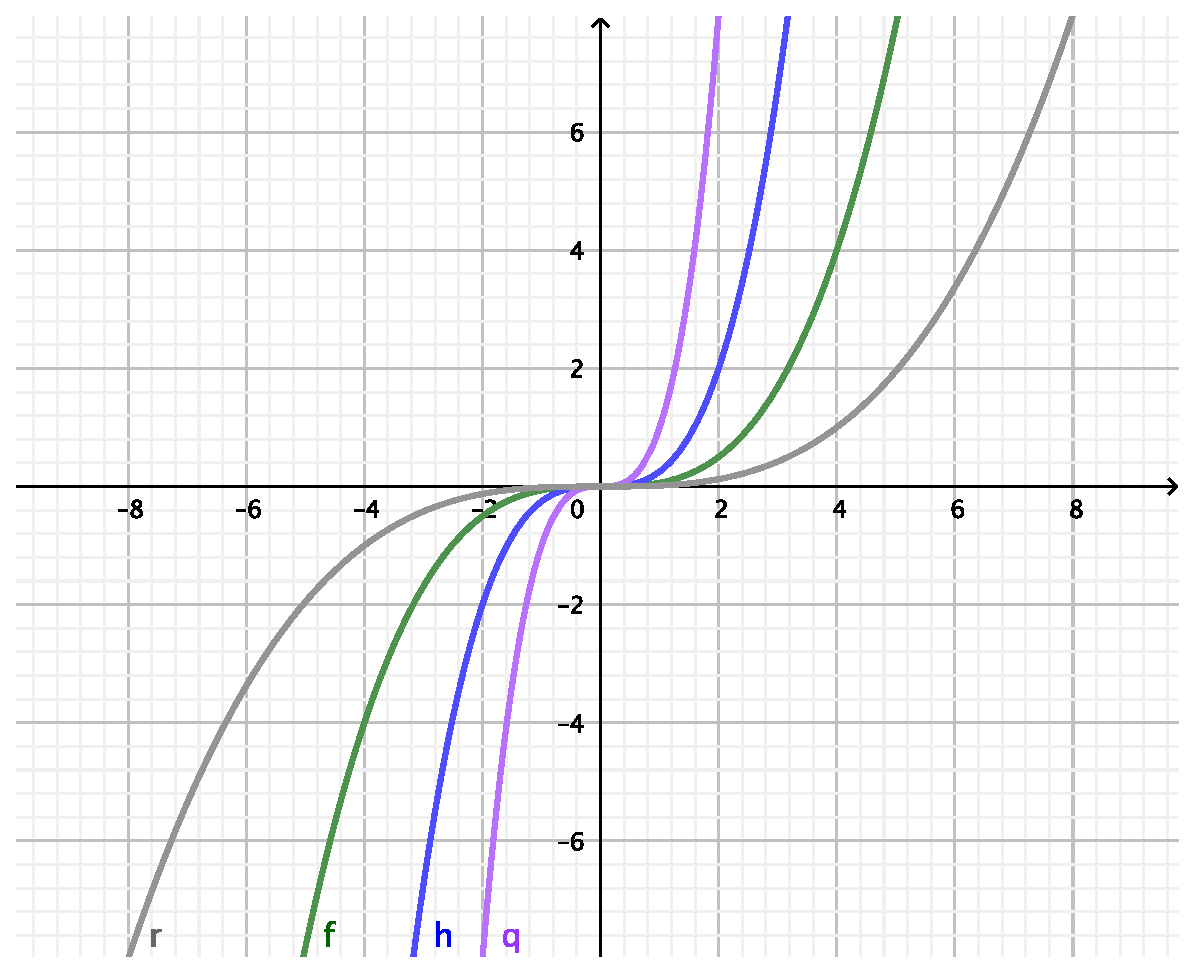
\includegraphics[height=12\baselineskip]{kap3/BundelFunktionenscharen.eps}
\end{minipage}
